\documentclass[crop,tikz,border=1px]{standalone}

\usetikzlibrary{arrows,positioning,scopes,automata,calc,chains}

\begin{document}
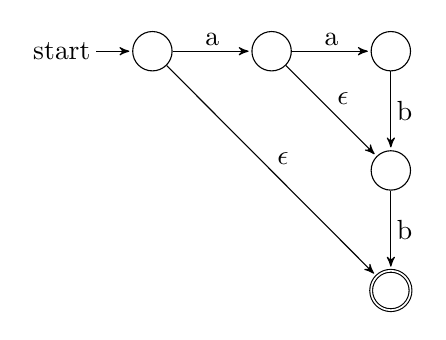
\begin{tikzpicture}[->,>=stealth',shorten >=1pt,auto,node
  distance=1cm,inner sep=2pt,start chain=going right,
  mystate/.style={state,text centered,minimum size=.5cm,on chain}]

  \node[initial,mystate] (q0) {};
  \node[mystate] (q1) [right=of q0] {};
  \node[mystate] (q2) [right=of q1] {};
  \node[mystate] (q3) [below=of q2] {};
  \node[mystate,accepting] (q4) [below=of q3] {};

  \draw (q0) edge node {a} (q1)
        (q1) edge node {a} (q2)
        (q2) edge node {b} (q3)
        (q3) edge node {b} (q4)
        (q1) edge node {\(\epsilon\)} (q3)
        (q0) edge node {\(\epsilon\)} (q4);

\end{tikzpicture}
\end{document}
